%Results and Discussion


For the first section of the results, ideas were assigned randomly onto the nodes of four different network structures (caveman, small world, random, and scale-free). Chapter 4 describes the network structures and idea distributions that are discussed. Simulations were run for each network structure for 27 different parameter combinations (three values for each of $\phi$, $\delta$ and $\alpha$). The effects of each network structure on the idea distribution was evaluated on five features: the average dominance time of dominant (i.e., most frequent) ideas, the novelty index, the intra-idea distance, the neighbourhood index, and the frequency of dominance of an idea (see Table \ref{Tab2}). We also investigated how these effects varied with the three parameters ($\phi$, $\delta$, $\alpha$).

The second section of the results investigated the opposite direction of effects: how changing the idea distribution affected the resulting network structure. To do this we applied three different idea distributions (random, parallel, and anti-parallel to the structure) to a caveman network (see Table \ref{Tab2}) with 40 caves. There were again 27 different parameter combinations for each idea distribution, as in the previous analysis. The five features of the network structure that we evaluated were: the clustering coefficient, the degree distribution of the nodes, the number of connected components, the average path length, and the network diameter. 

We found that there were different behaviours for some features of the idea distribution depending on the network structure, and that there were different behaviours for the structure features depending on the idea distribution. Both of these results were at least partly influenced by the values of $\phi$, $\delta$, and $\alpha$.

\subsection{Effects of Network Structure on Idea Distribution}

The results of the average dominance time and the novelty index were too dependent on the parameter values and were not included; the network structure does not seem to play a strong enough role over all parameter combinations in influencing these two features. It is not surprising, however, that the novelty index was highly dependent on the value of $\alpha$, but it is not so intuitive why the average dominance time was not correlated with $\alpha$ at all: increasing the number of novel ideas decreases the possible number of `followers' for already-established ideas, which should affect the frequency of dominance and therefore the dominance time. Perhaps the value of $\alpha$ would need to be increased to observe this behaviour.

Furthermore, we observed two different results for the intra-idea distance and the neighbourhood index: those from the caveman and small world structures, and those from the random and scale-free structures. All three parameter values affected these results. 


\subsubsection{Intra-Idea Distance and Neighbourhood Index}

For any parameter combination, the caveman and small world structures resulted in larger intra-idea distances (respectively) than those of the random and scale-free structures, which were very similar to each other (Figure \ref{fig1}). Interestingly, a similar influence was found on the neighbourhood index: the caveman structure held the largest index regardless of parameter combination, followed by the small world, random, and scale-free structures (Figure \ref{fig1}). It seems that the caveman structure encourages nodes to be within the direct neighbourhood of like-minded nodes (nodes with the same idea) and at a farther distance from like-minded nodes that are not in their direct neighbourhood, whereas the random and scale-free structures have a tendency to keep like-minded nodes in each other's direct neighbourhood but to also keep those like-minded nodes not in their direct neighbourhood at a shorter distance. The difference in intra-idea distance between network structures could be a result of the general smaller average path distance that random and scale-free networks have as compared to the caveman and small world graphs.

\begin{figure}
[htp]
\begin{center}
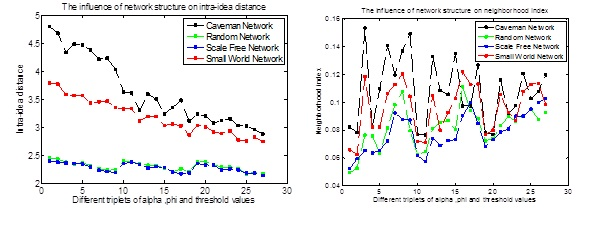
\includegraphics{Fig1}
\end{center}
\caption{The influence of network structure on intra idea distance (left) and neighborhood index (right) for 27 distinct sets of parameters (triplets of alpha-phi-threshold).}
\label {fig1}
\end{figure}


\paragraph{Dependence on $\alpha$}
For all network structures, increasing the level of innovation $\alpha$ decreased the intra-idea distance. This effect was more pronounced in the scale-free and random networks (Figure \ref{fig3}). Does innovation bring people together in scientific communities? Perhaps, and perhaps not. It is possible that these results are due to the construction of our model: because the mechanism of influence involves complex contagion, new ideas would not be able to spread (since they are held only by the originator) and therefore these ideas would technically have an intra-idea distance of zero.

\begin{figure}
[htp]
\begin{center}
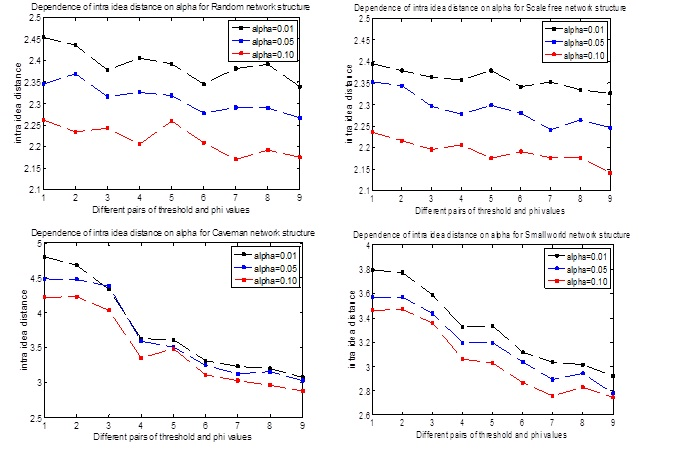
\includegraphics{Fig3}
\end{center}
\caption{Dependence of intra idea distance on alpha for each network structure. Horizontal axis corresponds to distinct pairs of phi-threshold and vertical axis is the intra idea distance. Each curve corresponds to a different value of alpha. Black curve corresponds to the smallest value of alpha and it always has the highest intra idea distance while the red curve corresponds to the largest value of alpha which always has the lowest value of intra idea distance.}
\label {fig3}
\end{figure}

Higher values of $\alpha$ also increased the neighbourhood index for all network structures. This correlation was again most visible for the scale-free network, followed by the random network (Figure \ref{fig4}). One possible explanation for this correlation is that the more novel ideas nodes create, the less likely it is that the contagion threshold is met for other ideas, and thus nodes will only be rewiring instead of also changing their ideas. Thus more like-minded nodes will be connected, and the index increases. 

\begin{figure}
[htp]
\begin{center}
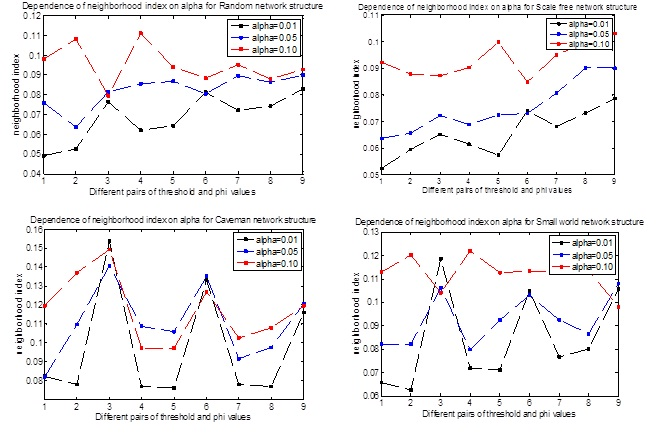
\includegraphics{Fig4}
\end{center}
\caption{Dependence of neighborhood index on alpha for each network structure. Horizontal axis corresponds to distinct pairs of phi-threshold and   vertical axis is the neighborhood index. Each curve corresponds to a different value of alpha. Red curve corresponds to the largest value of alpha and it has the highest neighborhood index while the black curve corresponds to the smallest value of alpha which has the lowest value of intra idea distance.}
\label {fig4}
\end{figure}

\paragraph{Dependence on $\phi$}
By increasing $\phi$, the intra-idea distance decreased for all network structures. This correlation is quite an intuitive result since $\phi$ is the probability of deleting a connection between two nodes with different ideas and the formation of a new connection between two nodes with the same idea, and thus, by increasing $\phi$ the distance between like-minded nodes decreases. Unlike the $\alpha$ parameter, the effects of $\phi$ are more pronounced for the caveman and small world structures rather than for the random and scale-free networks (Figure \ref{fig5}).

\begin{figure}
[htp]
\begin{center}
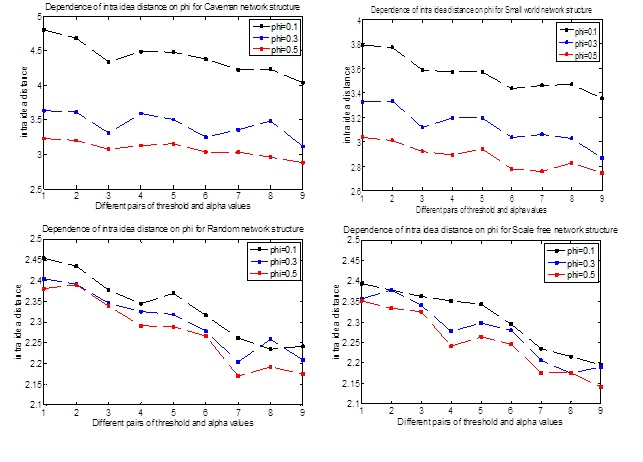
\includegraphics{Fig5}
\end{center}
\caption{Dependence of intra idea distance on phi for each network structure. Horizontal axis corresponds to distinct pairs of alpha-threshold and   vertical axis is the intra idea distance. Each curve corresponds to a different value of phi. Black curve corresponds to the smallest value of phi and it always has the highest intra idea distance while the red curve corresponds to the largest value of phi which always has the lowest value of intra idea distance.}
\label {fig5}
\end{figure}

On the other hand, the effects of $\phi$ on the neighborhood index varied between networks. Increasing $\phi$ increased the neighbourhood indexes of the random and scale-free networks, while it decreased the neighbourhood index of the caveman network and had no correlation with changes in the small world network (Figure \ref{fig6}).

\begin{figure}
[htp]
\begin{center}
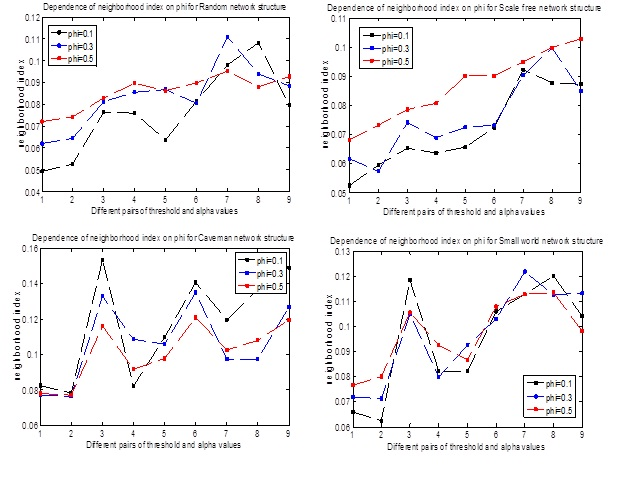
\includegraphics{Fig6}
\end{center}
\caption{Dependence of neighborhood index on phi for each network structure. Horizontal axis corresponds to distinct pairs of alpha-threshold and   vertical axis is the neighborhood index. Each curve corresponds to a different value of phi. Increasing phi leads to increase neighborhood distance for Random and Scale free networks while increasing phi causes the neighborhood index to be decreased for Cavemen Network. For Small world network there is no significant dependence of neighborhood index on phi.}
\label {fig6}
\end{figure}

\paragraph{Dependence on $\delta$}
Increasing values of the complex contagion threshold $\delta$ slightly decreased the intra-idea distance for the caveman and small world network structures (Figure \ref{fig7}). 

\begin{figure}
[htp]
\begin{center}
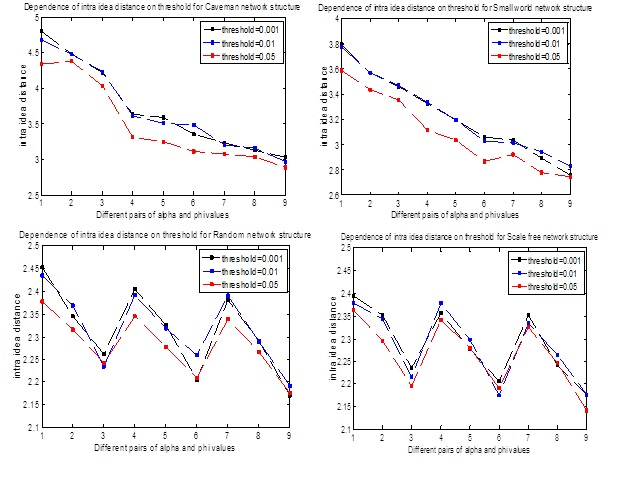
\includegraphics{Fig7}
\end{center}
\caption{Dependence of intra idea distance on complex contagion threshold for each network structure. Horizontal axis corresponds to distinct pairs of alpha-phi and   vertical axis is the intra idea distance. Each curve corresponds to a different value of complex contagion threshold. Black curve corresponds to the smallest value of complex contagion threshold and it has the highest intra idea distance while the red curve corresponds to the largest value of complex contagion threshold which has the lowest value of intra idea distance.}
\label {fig7}
\end{figure}

No correlation was found between the neighbourhood index of the small world, scale-free, and random network structures and values of $\delta$. However, the neighbourhood index for the caveman network increased as $\delta$ increased (Figure \ref{fig8}). This is an interesting result. On one hand, it is intuitive since requiring more like-minded nodes to be in the direct neighbourhood for a node to adopt their idea automatically increases the number of like-minded nodes in the neighbourhood (if the node adopts their idea). However, increasing $\delta$ could have the opposite effect: if the threshold is too high, nodes will not adopt their neighbhours' ideas and thus the neighbourhood index would remain small. The influence of $\delta$ only on the caveman network could be due to this structure's higher degree per node: almost all nodes have the same degree, whereas the other structures have the same average amount but with greater variance.

\begin{figure}
[htp]
\begin{center}
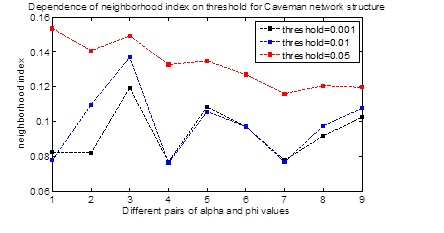
\includegraphics{Fig8}
\end{center}
\caption{Dependence of neighborhood index on complex contagion threshold. Horizontal axis corresponds to distinct pairs of alpha-phi and vertical axis is neighborhood index. Each curve corresponds to a different value of complex contagion threshold. Red curve corresponds to the largest value of complex contagion threshold which has the largest value of neighborhood index while black curve corresponds to the smallest value of complex contagion threshold and it has the smallest neighborhood index.}
\label {fig8}
\end{figure}


\subsubsection{Frequency of Dominance}

This feature is interesting if one considers scientific society. How dominant are dominant ideas in the scientific community? Does the structure of the community influence this dominance? For all parameter combinations and for all network structures in our simulations, the frequency of dominance of ideas increased with time. This may suggest that none of these structures impede the adoption of new ideas. More surprisingly, however, the increase in dominance frequency progressed more quickly for the caveman network structure (Figure \ref{fig2}). Could it be that this structure encourages nodes to adopt dominant ideas more easily? This may not be generalizable because the results are quite sensitive to parameter values due to the stochasticity of the simulations. For example, Figure \ref{fig2} shows a different combination of parameters, and here the faster increase in the dominance is not observed for the caveman structure.

\begin{figure}
[htp]
\begin{center}
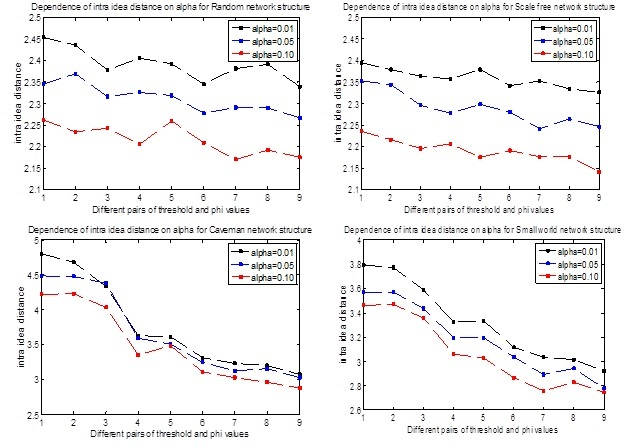
\includegraphics{Fig2}
\end{center}
\caption{Frequency of the dominant idea at each time for four distinct network structures and two different sets of parameters: phi=0.5, alpha=0.01, threshold=0.05 (top) and phi=0.3, alpha=0.1, threshold=0.05 (bottom).}
\label {fig2}
\end{figure}




\subsection{Effects of Idea Distribution on Network Structure}


We observed that the results of applying a parallel idea distribution on the features of the network structure were quite different to the results of the random and anti-parallel idea distributions. It is interesting that for all parameter combinations and for each idea distribution, the network always remained fully connected. This could be because of the nature of our model: in order to disconnect with one node, there must be another node with the same idea to connect with. The nodes in a caveman network structure are, in a sense, `saturated' since they are fully connected to their caves, and thus they remain connected to at least one of their original cave members. 

While the networks always remained fully connected (Figure \ref{fig9}), the remaining features changed. These effects did not change with the parameter $\alpha$ for any of the idea distributions (see Figure \ref{fig11}, Figure \ref{fig12} and Figure \ref{fig13}). Given these simulation results, perhaps a caveman-structured scientific community would also manage certain levels of innovativity without changing its fundamental structure.

\begin{figure}
[htp]
\begin{center}
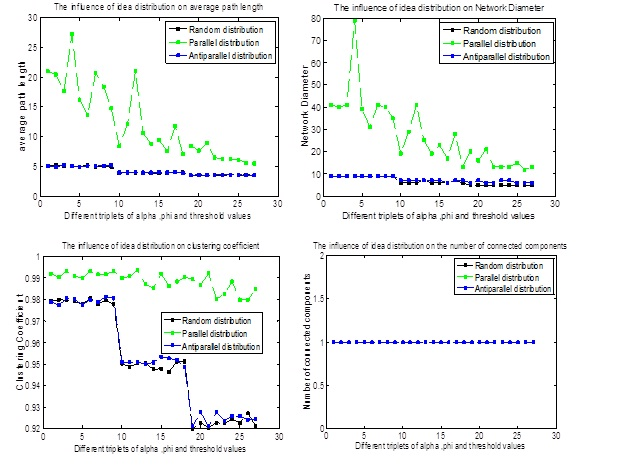
\includegraphics{Fig9}
\end{center}
\caption{The influence of idea distribution on average path length (upper left), network diameter (upper right), clustering coefficient (bottom left) and number of connected components (bottom right) for 27 distinct sets of parameters (triplets of alpha-phi-threshold). }
\label {fig9}
\end{figure}

\begin{figure}
[htp]
\begin{center}
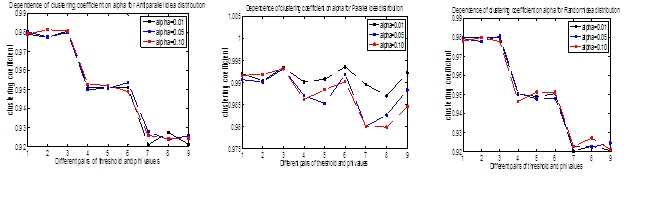
\includegraphics{Fig11}
\end{center}
\caption{ Dependence of clustering coefficient on alpha for each idea distribution. Horizontal axis corresponds to distinct pairs of phi-threshold and   vertical axis is the clustering coefficient. Each curve corresponds to a different value of alpha. There is no dependence on alpha for clustering coefficient of the networks with any idea distribution.}
\label {fig11}
\end{figure}\begin{figure}
[htp]
\begin{center}
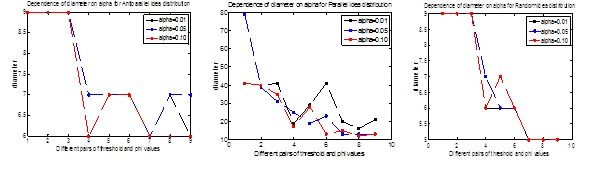
\includegraphics{Fig12}
\end{center}
\caption{ Dependence of network diameter on alpha for each idea distribution. Horizontal axis corresponds to distinct pairs of phi-threshold and vertical axis is the network diameter. Each curve corresponds to a different value of alpha. There is no dependence on alpha for the diameters of the networks with any idea distribution}
\label {fig12}
\end{figure}\begin{figure}
[htp]
\begin{center}
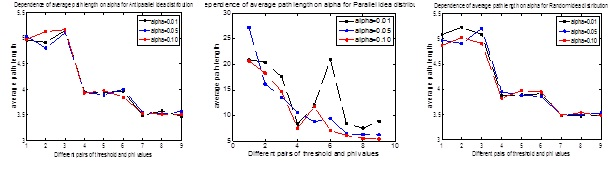
\includegraphics{Fig13}
\end{center}
\caption{Dependence of average path length on alpha for each idea distribution. Horizontal axis corresponds to distinct pairs of phi-threshold and   vertical axis is the average path length. Each curve corresponds to a different value of alpha. There is no dependence on alpha for average path length of the networks with any idea distribution.}
\label {fig13}
\end{figure}


\subsubsection{Clustering Coefficient}

The clustering coefficient of resulting networks varied with the type of idea distribution. When nodes in the same cave shared the same idea (parallel distribution), the clustering coefficient was larger (Figure \ref{fig10}). Additionally, the clustering coefficients for both the random and the anti-parallel idea distributions decreased in a similar manner regardless of the parameter combinations. Both of these results are intuitive since less rewiring would have taken place for the parallel distribution case, and the high clustering coefficient of the caveman structure would have been conserved, whereas more rewiring would have ocurred for the two other distributions, thus decreasing the clustering coefficients.

\begin{figure}
[htp]
\begin{center}
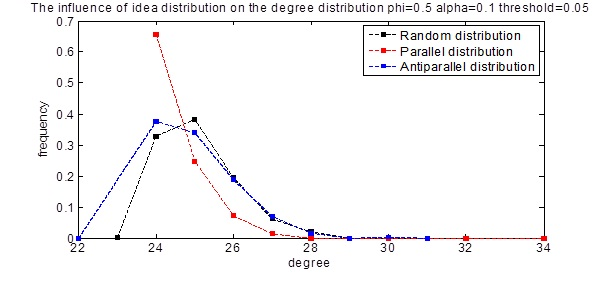
\includegraphics{Fig10}
\end{center}
\caption{ The influence of idea distribution on the degree distribution of the network. Horizontal axis corresponds to the degree of the nodes and vertical axis corresponds to the relative frequency of the nodes with that certain degree.   }
\label {fig10}
\end{figure}

\paragraph{Dependence on parameters}
Increasing values of the rewiring parameter $\phi$ decreased the clustering coefficient for all starting distributions, especially for the random and anti-parallel distributions (Figure \ref{fig16}). This again is intuitive since $\phi$ increases the chances of changing connections in a highly clustered network.
Increasing values of $\delta$, however, only slightly increased the clustering coefficient when using a parallel idea distribution (Figure \ref{fig19}). 

\begin{figure}
[htp]
\begin{center}
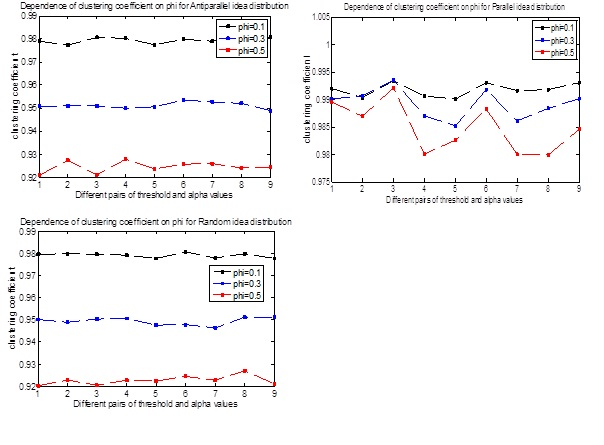
\includegraphics{Fig16}
\end{center}
\caption{Dependence of average path length on phi for each idea distribution. Horizontal axis corresponds to distinct pairs of alpha-threshold and vertical axis is the average path length. Each curve corresponds to a different value of phi. }
\label {fig16}
\end{figure}

\begin{figure}
[htp]
\begin{center}
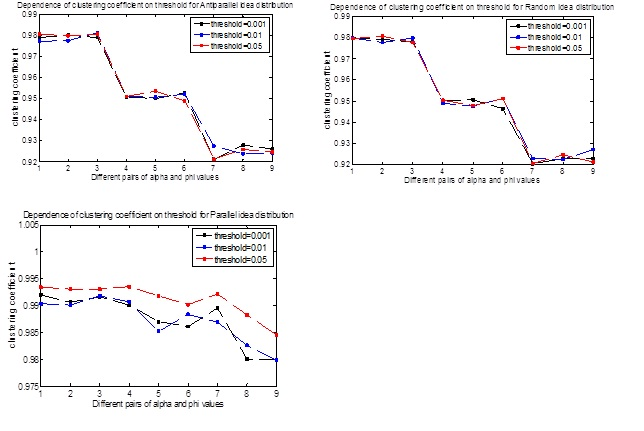
\includegraphics{Fig19}
\end{center}
\caption{Dependence of clustering coefficient on complex contagion threshold for each idea distribution. Horizontal axis corresponds to distinct pairs of phi-alpha and   vertical axis is the clustering coefficient. Each curve corresponds to a different value of complex contagion threshold.}
\label {fig19}
\end{figure}

\subsubsection{Average Path Length}
The average path length of resulting networks was larger when a parallel idea distribution was used (Figure \ref{fig9}). This is not surprising, since the structure of the caveman network was more preserved (because most nodes were already connected to like-minded nodes and did not need to rewire), and its average path length is larger than that of more randomized networks, such as the ones resulting from a larger amount of rewiring. 
\paragraph{Dependence on parameters}
Increasing $\phi$, regardless of the idea distribution, decreased the average path length. This effect was more prononced for the random and anti-parallel idea distribution cases (Figure \ref{fig14}). This is another intuitive result since more rewiring naturally disturbs the rigid structure of a caveman network, thereby decreasing its large average path length; rewiring also occurs less frequently in the parallel idea distribution case because most nodes are already connected to like-minded nodes.
Changing values of $\delta$ (which requires more than one neighbouring node to have the same idea in order to influence the chosen node) did not change the effects of idea distributions on the average path length (Figure \ref{fig17}). This is natural, since nodes were either already connected to a significant number of nodes with the same idea (in the case of the parallel distribution), not connected to any other node with the same idea (the anti-parallel case), or connected to nodes with random assignment of ideas. Thus the threshold $\delta$ would either already be fulfilled from the start, would definitely not be fulfilled, or would have a very small chance of being fulfilled, respectively.

\begin{figure}
[htp]
\begin{center}
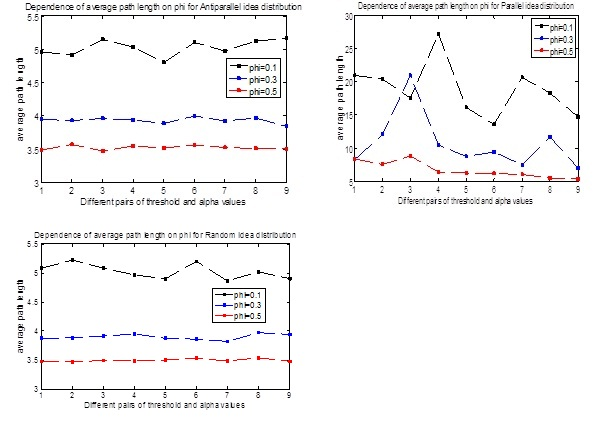
\includegraphics{Fig14}
\end{center}
\caption {Dependence of clustering coefficient on phi for each idea distribution. Horizontal axis corresponds to distinct pairs of alpha-     threshold and   vertical axis is the clustering coefficient. Each curve corresponds to a different value of phi.}
\label {fig14}
\end{figure}

\begin{figure}
[htp]
\begin{center}
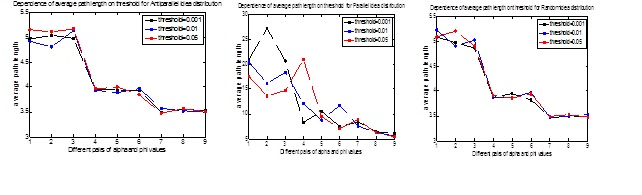
\includegraphics{Fig17}
\end{center}
\caption{ Dependence of average path length on complex contagion threshold for each idea distribution. Horizontal axis corresponds to distinct pairs of alpha-phi and vertical axis is the average path length. Each curve corresponds to a different value of complex contagion threshold. There is no dependence on complex contagion for average path length with any idea distribution.}
\label {fig17}
\end{figure}


\subsubsection{Network Diameter}
Similar to the clustering coefficient and the average path length, the network diameter was larger when the parallel idea distribution was applied (Figure \ref{fig9}). This distribution encouraged the structure of the caveman network to remain mostly unchanged, and thus the farthest distance between two nodes was larger than for the case of random or anti-parallel distributions, where more rewiring occured. 
\paragraph{Dependence on parameters}
As $\phi$ increased, the network diameter decreased for all idea distributions, and slightly less for the parallel distribution (Figure \ref{fig15}). Rewiring a caveman network intuitively may decrease the network diameter by connecting more of its caves.
Similar to the average path length, values of $\delta$ did not change the behaviour of the network diameter given the idea distributions (Figure \ref{fig18}).

\begin{figure}
[htp]
\begin{center}
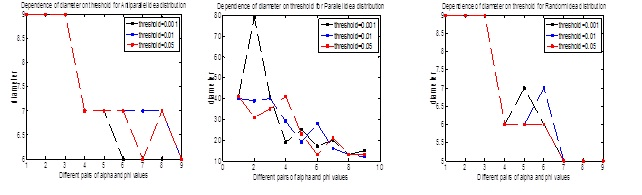
\includegraphics{Fig18}
\end{center}
\caption{ Dependence of network diameter on complex contagion threshold for each idea distribution. Horizontal axis corresponds to distinct pairs of phi-alpha and vertical axis is the network diameter. Each curve corresponds to a different value of complex contagion threshold. There is no dependence on complex contagion for network diameter with any idea distribution.}
\label {fig18}
\end{figure}

\begin{figure}
[htp]
\begin{center}
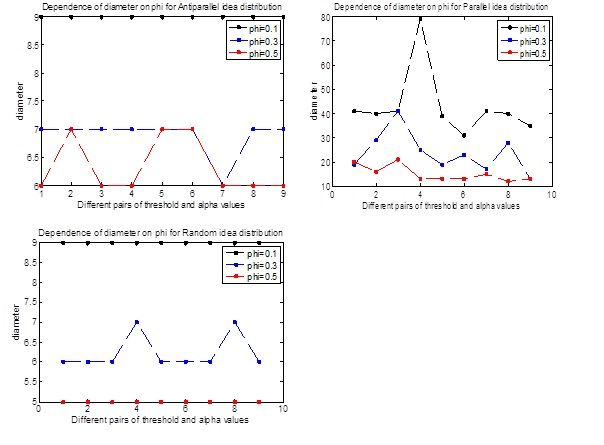
\includegraphics{Fig15}
\end{center}
\caption {Dependence of network diameter on phi for each idea distribution. Horizontal axis corresponds to distinct pairs of alpha-threshold and vertical axis is the network diameter. Each curve corresponds to a different value of phi. }
\label {fig15}
\end{figure}




\subsubsection{Degree Distribution}
Random graphs have a somewhat normally distributed degree distribution. Scale-free graphs, on the other hand, have a degree distribution that follows a scale-free power-law. We observed that the degree distribution of the networks depended on the idea distribution (Figure \ref{fig10}). A parallel idea distribution resulted in a degree distribution similar to that of a scale-free graph, which is not surprising. Caveman graphs have two or three different degrees for their nodes, and allowing for some rewiring would 'smooth' out this discrete distribution. Similar to previous results, the random and anti-parallel idea distributions behaved similarly: their degree distribution was similar to that of random graphs. It is interesting to see such a visible difference in these distributions over relatively few time steps (1000 steps), regardless of the parameter combinations. 


\subsection{Discussion}

As previously mentioned, we observed that some features of the idea distribution varied with the type of network structure. We also observed that some features of the network structure varied with the kind of idea distribution implemented. Some of these results were intuitive and expected, while others were not.

Network structure mainly influenced two features of the idea distribution: the intra-idea distance and the neighbourhood index. The intra-idea distance was larger for the caveman and small world networks, as anticipated. However, contrary to expectations, the neighbourhood index was larger for these two structures, and the caveman structure did not decrease the frequency of dominance (and neither did any other structure).  Additionally, the values of $\phi$ and $\delta$ did correlate with changes in the values of the intra-idea distance (by decreasing it) and the neighbourhood index (with different effects depending on the structure), but not always: $\delta$ did not vary the results of the intra-idea distance or the neighbourhood index of the random and scale-free networks, and $\phi$ did not vary the neighbourhood index in the small world network. Lastly, and also contrary to expectations, increasing the $\alpha$ values increased the neighbourhood index of networks.


Four of the five features of the network structure changed with different idea distributions. The connected component interestingly remained one, regardless of the idea distribution and parameter values. Feature values of the anti-parallel and random idea distributions differed from those of the parallel distribution. Most features changed as expected: the clustering coefficient, average path length, and network diameter were larger when the parallel idea distribution was used as compared to the other two, and their values were similar to those of a caveman network structure. The clustering coefficient of the anti-parallel idea distribution networks did decrease, as expected. The degree distribution did increase in variance (becoming more similar to a normal distribution) for the networks that were initiated with a random or anti-parallel idea distribution, but the degree distribution of the parallel idea distribution networks resembled that of a scale-free power law. Values of $\phi$ influenced the features of the random and antiparallel distribution networks the most. However, the structure features of the networks with the random idea distribution were not more sensitive to parameter values as would have been expected; they behaved similar to those of the networks with the anti-parallel idea distribution. Values of $\delta$ only correlated with changes in the clustering coefficient of the networks with a parallel idea distribution, and only weakly. Values of $\alpha$ did not correlated with any changes of feature values. 
